%% ============================================================
%%  SECCIÓN 4 — Fundamento Teórico
%% ============================================================

\section{Fundamento Teórico}
\label{sec:fundamento}

El osciloscopio es un instrumento electrónico de adquisición y representación gráfica que permite visualizar diferencias de potencial eléctrico en función del tiempo o de otra tensión eléctrica~\cite{serway}.

\begin{figure}[H]
    \centering
    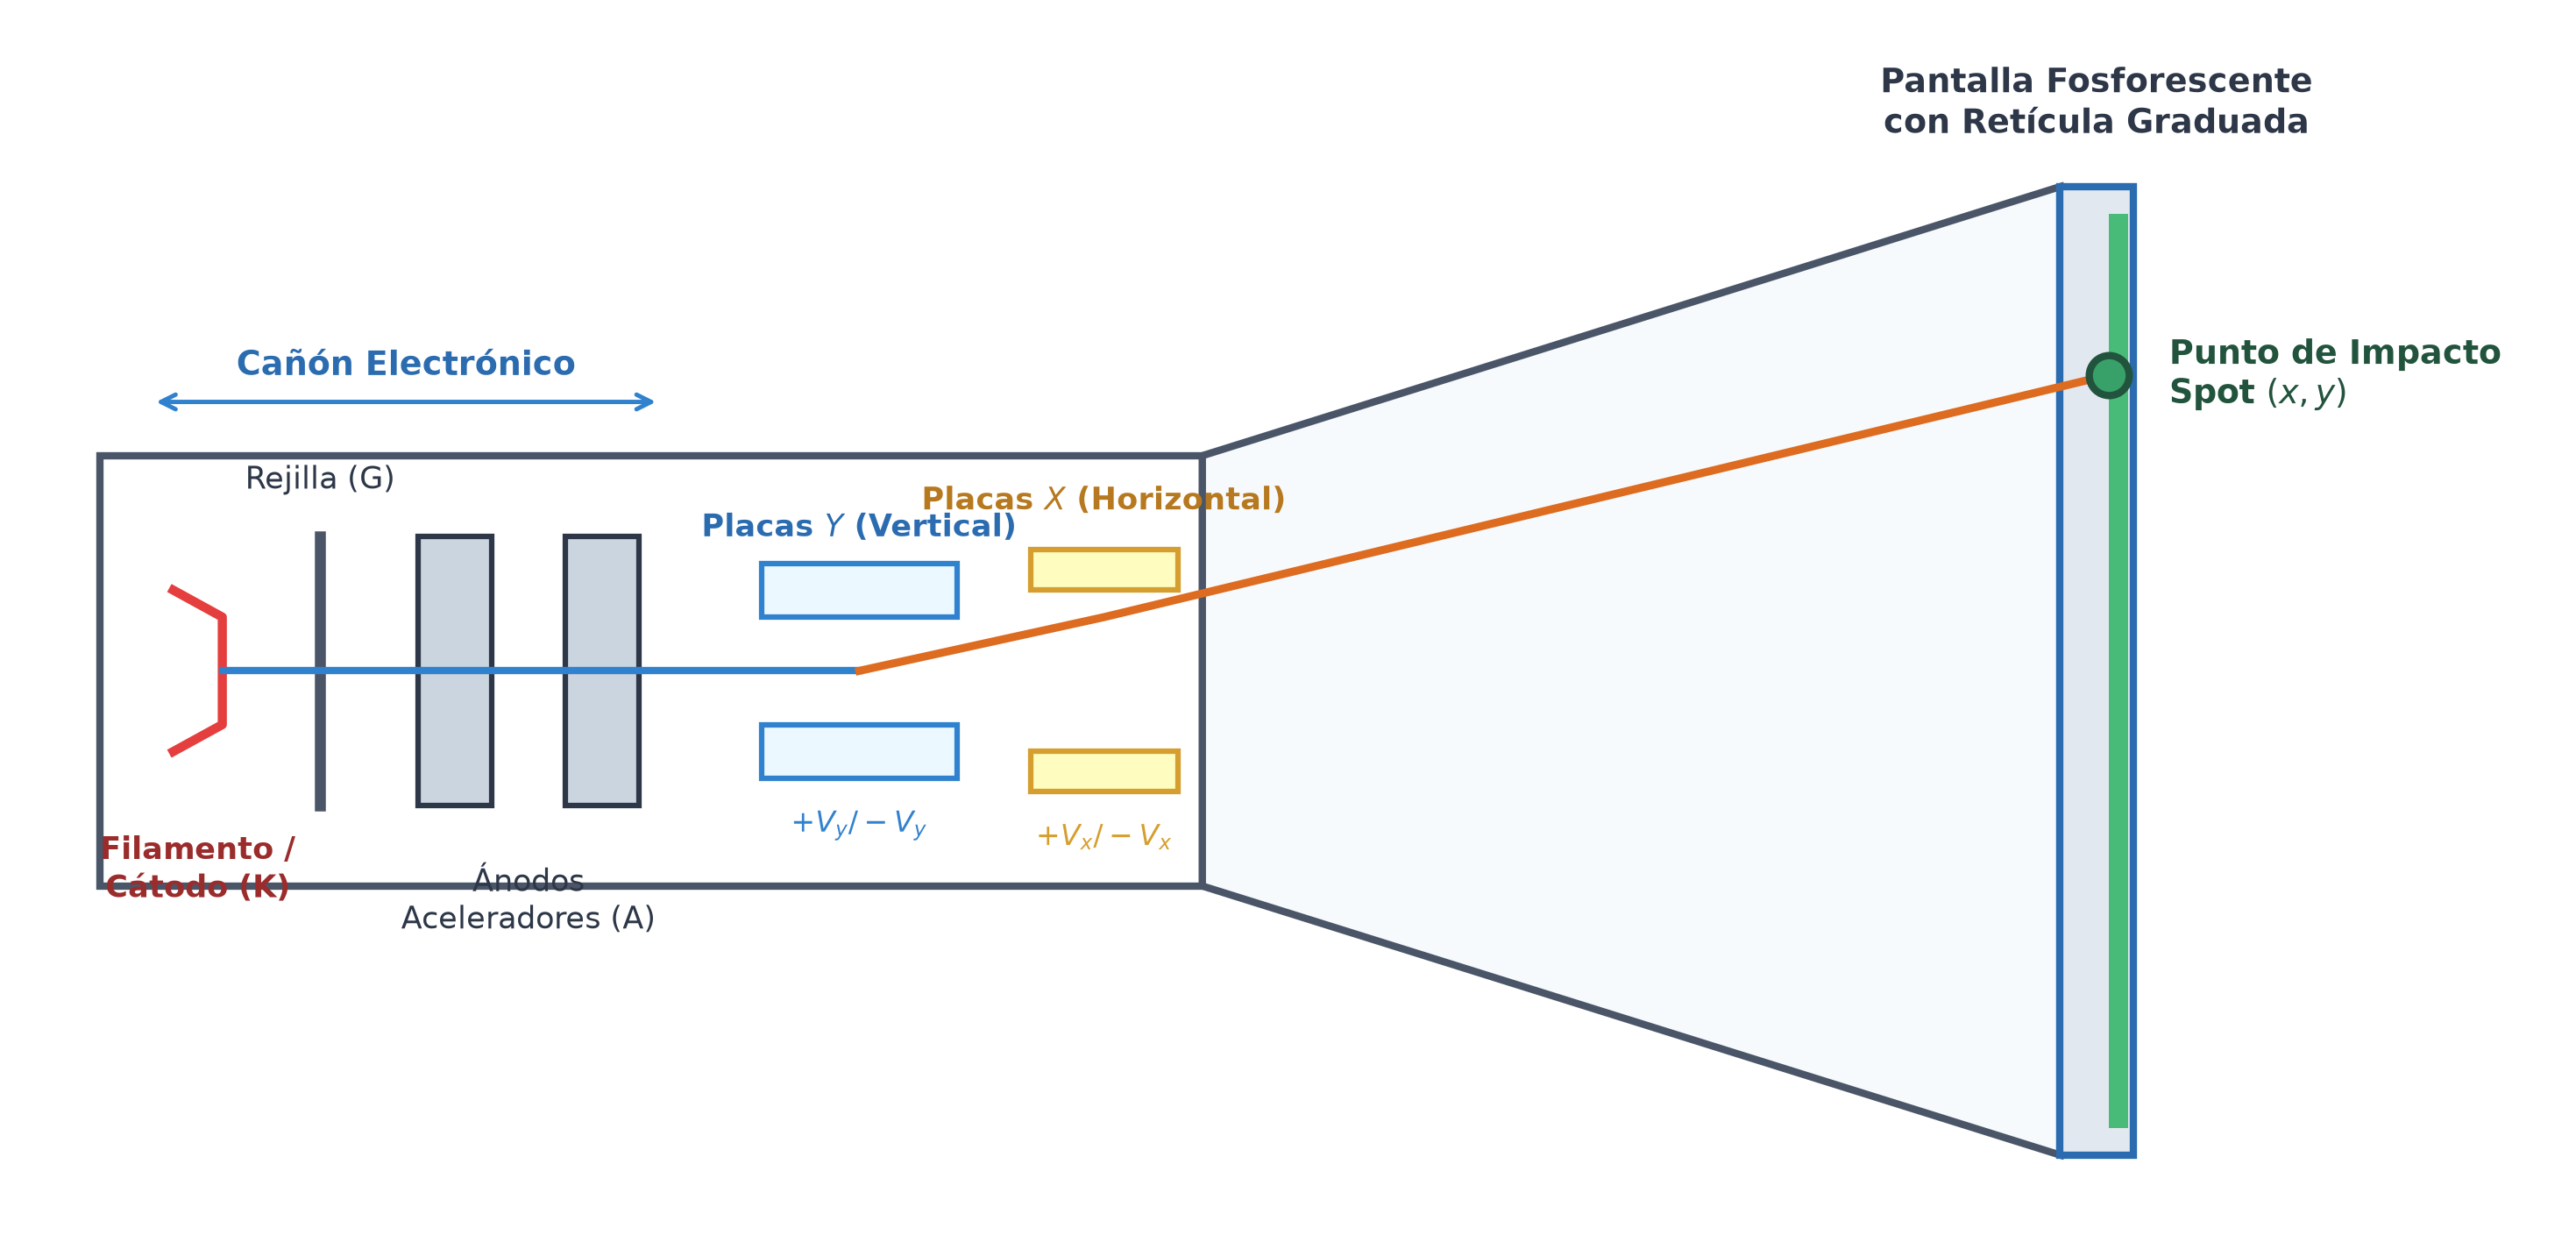
\includegraphics[width=0.85\linewidth]{fig_trc_esquema}
    \caption{Diagrama esquemático del Tubo de Rayos Catódicos (TRC) mostrando el cañón de electrones, los pares de placas deflectoras electrostáticas ortogonales ($X$ e $Y$) y la pantalla fosforescente graduada.}
    \label{fig:trc_esquema}
\end{figure}

\subsection{Principio de Adquisición y Escalas en Osciloscopios Digitales}
En un osciloscopio digital moderno (DSO), la señal continua de entrada $V(t)$ es acondicionada por un amplificador y atenuador programable de alta impedancia ($R_{\text{in}} = \qty{1}{\mega\ohm} \pm \qty{2}{\percent}$ en paralelo con $C_{\text{in}} = \qty{14 \pm 2}{\pico\farad}$) y posteriormente muestreada por un convertidor analógico-digital (ADC) de $8$ a $16\text{ bits}$ de resolución~\cite{rs_rtc1000_specs}.

La señal procesada se proyecta en una retícula ortogonal dividida en divisiones verticales ($Y$) y horizontales ($X$), tal como se ilustra en la Figura~\ref{fig:parametros_onda}. La tensión instantánea $V(t)$ y el tiempo $t$ se determinan mediante las relaciones fundamentales:
\begin{align}
    V(t) &= N_y(t) \cdot S_v \label{eq:voltaje_escala} \\
    t &= N_x \cdot S_t \label{eq:tiempo_escala}
\end{align}
donde $N_y$ es el número de divisiones verticales de deflexión desde la línea de referencia cero ($\text{GND}$), $S_v$ es la sensibilidad o factor de escala vertical (\unit{\volt\per\division}), $N_x$ es el número de divisiones horizontales a lo largo del eje temporal, y $S_t$ es la base de tiempo horizontal (\unit{\second\per\division}).

\begin{figure}[H]
    \centering
    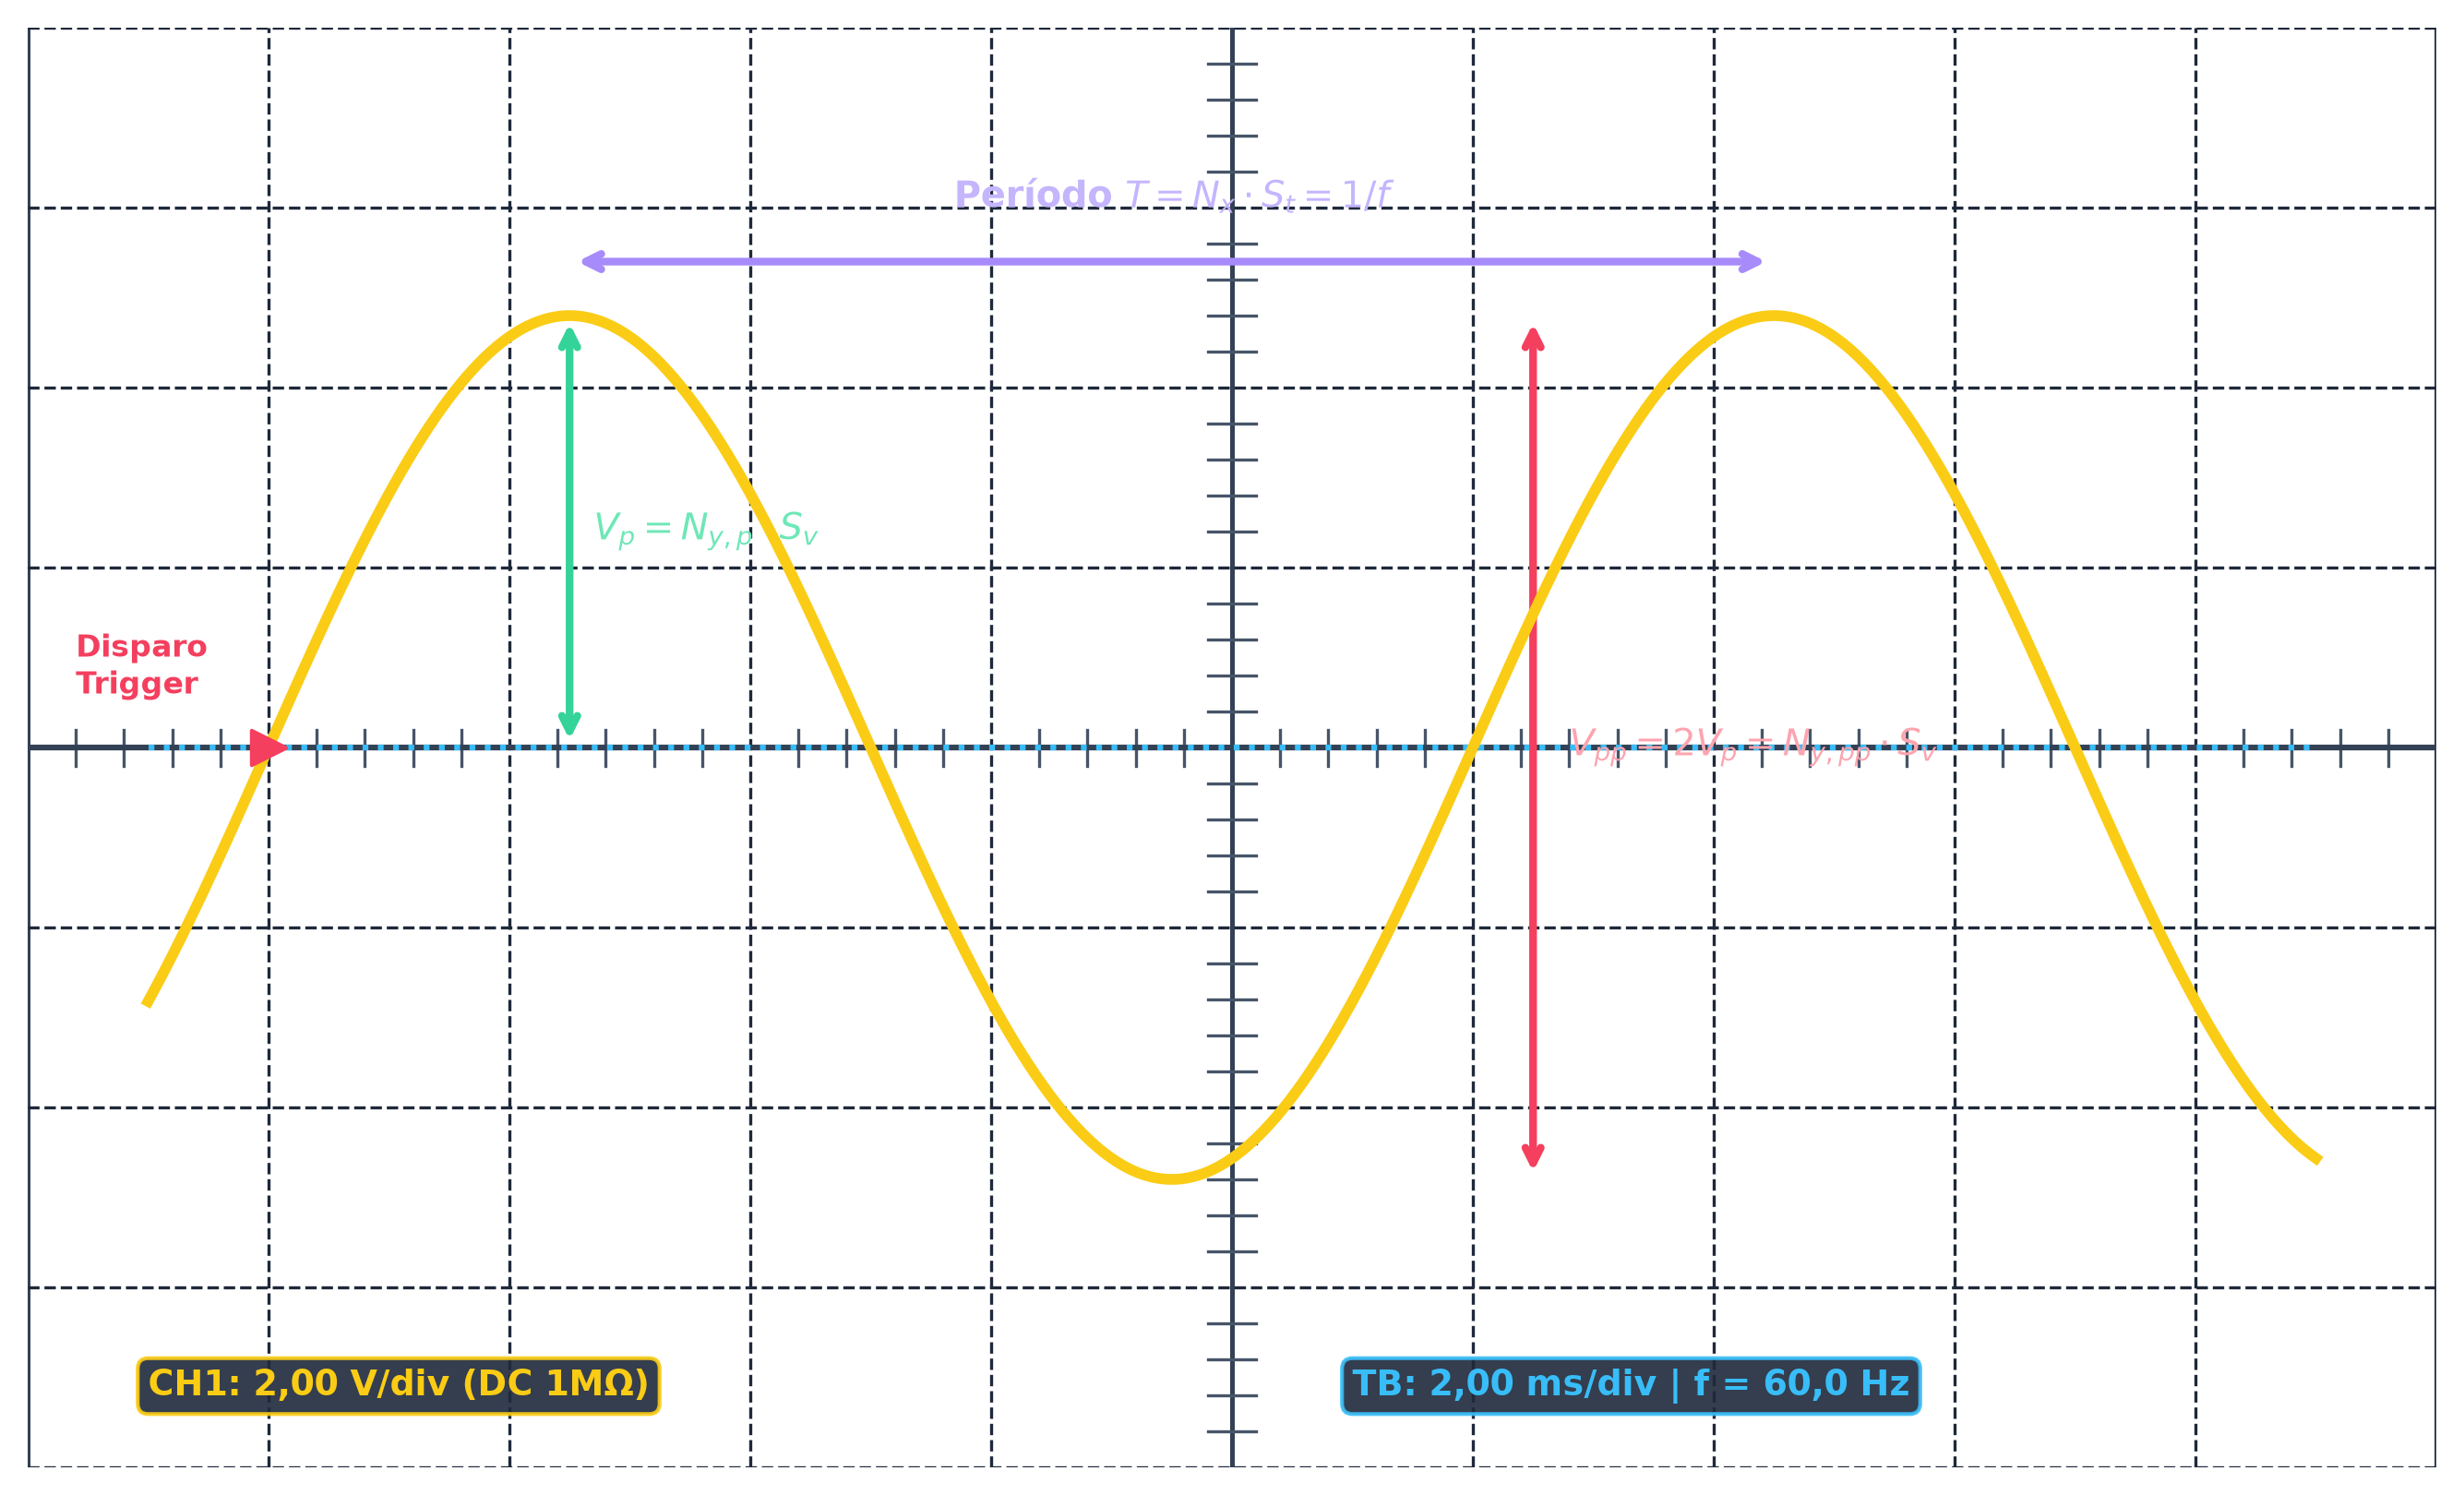
\includegraphics[width=0.85\linewidth]{fig_parametros_onda}
    \caption{Representación gráfica y anatomía de una señal periódica senoidal proyectada sobre la retícula del osciloscopio, destacando las cotas de amplitud pico ($V_p$), voltaje pico a pico ($V_{pp}$), período fundamental ($T$), línea de cero ($\text{GND}$) y nivel de disparo ($\text{Trigger}$).}
    \label{fig:parametros_onda}
\end{figure}

\subsection{Magnitudes Caracterizadoras de Señales Periódicas}
Una señal eléctrica periódica $V(t)$ satisface la condición $V(t + T) = V(t)$, donde $T$ es el período fundamental. La frecuencia $f$ representa el número de ciclos completos por segundo:
\begin{equation}
    f = \frac{1}{T} \label{eq:frecuencia}
\end{equation}
cuya unidad en el Sistema Internacional es el Hertz (\unit{\hertz} o \unit{\per\second}).

Para caracterizar la magnitud de una tensión alterna se definen tres parámetros esenciales:
\begin{enumerate}
    \item \textbf{Voltaje Pico ($V_p$ o Amplitud $V_0$):} Valor máximo positivo alcanzado por la señal respecto a su nivel medio de continua ($V_{\text{DC}}$):
    \begin{equation}
        V_p = \max[V(t)] - V_{\text{DC}} \label{eq:voltaje_pico}
    \end{equation}
    \item \textbf{Voltaje Pico a Pico ($V_{pp}$):} Diferencia absoluta entre el valor máximo positivo y el valor mínimo negativo de la onda:
    \begin{equation}
        V_{pp} = \max[V(t)] - \min[V(t)] = 2 V_p \label{eq:voltaje_pp}
    \end{equation}
    \item \textbf{Voltaje Eficaz o RMS (\textit{Root Mean Square}):} Valor de tensión continua equivalente que disiparía la misma potencia térmica promedio sobre una resistencia pura $R$ en un período completo~\cite{halliday}:
    \begin{equation}
        V_{\text{rms}} = \sqrt{\frac{1}{T} \int_0^T V^2(t)\,\mathrm{d}t} \label{eq:voltaje_rms_def}
    \end{equation}
\end{enumerate}

\subsubsection{Voltaje Eficaz para Formas de Onda Estándar}
Evaluando la integral~\eqref{eq:voltaje_rms_def} para las distintas funciones periódicas utilizadas experimentalmente:
\begin{itemize}
    \item \textbf{Onda Senoidal Pura ($V(t) = V_p \sin(\omega t)$):}
    \begin{equation}
        V_{\text{rms}} = \sqrt{\frac{V_p^2}{T} \int_0^T \sin^2(\omega t)\,\mathrm{d}t} = \frac{V_p}{\sqrt{2}} \approx 0{,}7071\,V_p \label{eq:rms_seno}
    \end{equation}
    \item \textbf{Onda Triangular Simétrica ($V(t)$ lineal por tramos):}
    \begin{equation}
        V_{\text{rms}} = \sqrt{\frac{1}{T} \int_0^T \left(\frac{4 V_p}{T} t - V_p\right)^2\,\mathrm{d}t} = \frac{V_p}{\sqrt{3}} \approx 0{,}5774\,V_p \label{eq:rms_triang}
    \end{equation}
    \item \textbf{Onda Cuadrada Simétrica ($V(t) = \pm V_p$ con ciclo de trabajo del \qty{50}{\percent}):}
    \begin{equation}
        V_{\text{rms}} = \sqrt{\frac{1}{T} \int_0^T V_p^2\,\mathrm{d}t} = V_p \label{eq:rms_cuadrada}
    \end{equation}
\end{itemize}

\subsection{Modo Graficador \texorpdfstring{$X$-$Y$}{X-Y} y Figuras de Lissajous}
Al desacoplar la base de tiempo horizontal interna ($S_t$) y conectar simultáneamente dos señales armónicas independientes en los canales analógicos $\text{CH1}$ (eje horizontal $x$) y $\text{CH2}$ (eje vertical $y$), el osciloscopio describe una curva paramétrica en el plano bidimensional:
\begin{equation}
    \begin{cases}
        x(t) = A_x \sin(2\pi f_x t) \\
        y(t) = A_y \sin(2\pi f_y t + \phi)
    \end{cases} \label{eq:lissajous_param}
\end{equation}
donde $A_x, A_y$ son las amplitudes, $f_x, f_y$ son las frecuencias respectivas y $\phi$ es el desfase relativo.

La trayectoria resultante recibe el nombre de \textbf{Figura de Lissajous}. Si las frecuencias $f_x$ y $f_y$ guardan una razón de números enteros sencillos ($n_x, n_y \in \mathbb{N}$), la curva es cerrada y estacionaria, verificándose la relación de tangencias:
\begin{equation}
    \frac{f_y}{f_x} = \frac{N_{\text{tang,horizontal}}}{N_{\text{tang,vertical}}} \label{eq:lissajous_ratio}
\end{equation}
donde $N_{\text{tang,horizontal}}$ representa el número de puntos de tangencia con una recta horizontal superior/inferior, y $N_{\text{tang,vertical}}$ con una recta vertical lateral.

Para $f_x = f_y$ (relación $1:1$), la figura describe una elipse cuya ecuación cartesiana general es:
\begin{equation}
    \left(\frac{x}{A_x}\right)^2 + \left(\frac{y}{A_y}\right)^2 - 2\left(\frac{x}{A_x}\right)\left(\frac{y}{A_y}\right)\cos\phi = \sin^2\phi \label{eq:elipse_lissajous}
\end{equation}
Si $\phi = 0$, la elipse colapsa en una línea recta de pendiente positiva $y = \frac{A_y}{A_x} x$; si $\phi = \pi$, la pendiente es negativa. Al aplicar la función de inversión polar del canal 2 ($\text{CH2 INVERT}$, $y \to -y$), la figura sufre una reflexión especular respecto al eje horizontal $X$, invirtiéndose el signo de su pendiente.